%!TEX root = aaai2014.tex
\section{INTRODUCTION}

% The vision of intelligent interactive systems, including robots, continues to become more realistic with technological advances 

%Future applications \todo{which one?} for autonomous systems, including robots, bring them into human environments. These applications will often require the system to adapt to the users preferences and to be able tp acquire new skills by interacting with the human. To fully harness the potential of such technologies, users should be allowed to focus their attention on the aims and context of the interaction rather than the protocol and technical details of the interface. Hence, the systems should be able to take advantage of communication means that are natural and intuitive for the human partner.

% nicolescu2003natural

Interactive learning \cite{nicolescu2003natural,breazeal2004tutelage} aims at developing systems that can learn by practical interaction with the user and finds applications in a wide range of fields such as human-robot interaction, tutoring systems or human-machine interfaces.
This type of learning combines ideas of learning from demonstration \cite{argall2009survey}, learning by exploration \cite{sutton1998reinforcement} and tutor feedback \cite{kaplan2002robotic}. Under this approach the human teacher interacts with the machine and provides extra feedback or guidance. 

% In addition, the device can act to improve its learning efficiency.
Approaches have considered: extra reinforcement signals \cite{thomaz2008teachable}, action requests \cite{lopes2009active}, disambiguation among actions \cite{chernova2009interactive}, preferences among states \cite{mason2011robot}, iterations between practice and user feedback sessions \cite{judah2010reinforcement}, and choosing actions that maximize the user feedback \cite{knox2009interactively}. 

A usual assumption in such systems is that the learner and the teacher share a mutual understanding of the meaning of each others' signals, and in particular the learning agent is usually assumed to know how to interpret teaching instructions from the human. In practice, this problem is solved due to two simplifications. On the one hand, the range of accepted instructions is limited to those predefined by the system developer. This approach, commonly used in human-robot interaction, lacks flexibility and adaptation to user specificities and, consequently, may not be well accepted by non-experts users with different preferences. 
%
On the other hand, sometimes it is not enough to predefine the instruction sets and it is necessary to perform a calibration phase to map raw signals such as speech or brain activity to their meanings. This is usually done using an ad-hoc protocol to collect labeled samples of the user instruction signals. This process must be well controlled to ensure signals are associated to the true intended meaning of the user.

The previous engineering solution is needed due to the chicken egg nature of the problem. In order to teach a system a new skill, it needs to understand the human instructions. And, in order to understand this feedback, the system must have some interaction with the human (e.g. through a controlled task as done in the calibration process) to learn what the instructions mean. 
%Consequently it is impossible for a user to instruct --- from scratch --- a machine using his own preferred teaching signals. 
Few works have studied and developed interactive learning systems that can learn both the meaning of signals and the task simultaneously. In human-robot interaction Griffiths et al. \cite{griffiths2012bottom} conducted an experiment with humans learning the meaning of unknown symbolic teaching signals. Lopes et al. \cite{macl11simul} presented sequential task experiments considering symbolic teaching signals and requiring a bootstrap with known signals. Grizou et al. \cite{grizou2013robot} extended their system for non-symbolic teaching signals while removing the need for bootstrapping with known signals. Which they later extended to non-invasive brain-computer interfaces (BCIs), proposed an uncertainty measure on both the task and the signal model for efficient planning, and performed online experiments \cite{grizou2014calibration}. Also, for P300 spellers, Kindermans et al. have shown that it is possible to exploit the repetition of signals \cite{Kindermans2012a} together with prior information (language models, information from other subjects) \cite{kindermans2014integrating} to calibrate the EEG decoder while using the speller. They exploit the particular fact that only one event out of six encodes a P300 potential in the speller paradigm. BCIs usually require user-dependent calibration and have to deal with the EEG brain signals non-stationarities. These facts, together with the poor signal-to-noise ratio of the EEG, make the EEG self-calibration one of the most challenging ones. 

 %Our approach differs by considering uncertainty reduction planning methods.
 %Our approach differs by the sequential nature of the task, the ability to estimate confidence on current belief and to plan actions efficiently.

%\todo{Following paragraph must be shortened}
%We believe solving this problem is useful for nowadays and future scenarios. For instance brain-computer interfaces (BCIs) are systems capable of decoding neural activity in real time, thereby allowing a machine to be directly controlled by thought. Such interfaces must be highly customized to adapt to each user brain signals. It requires a fastidious calibration procedure, where the user is asked to repeat hundreds of time the same thought process in order to collect labeled data. Moreover some signals change on a daily basis and calibration must be done again. Nowadays calibration procedure requires an expert to collect and train the classifier that will be use for during interaction, which in practice limits the use of EEG based system to labs or hospitals. A systems that would self-calibrated and adapt to each particular is an interesting may enable BCI technologies to go out of the labs. The same problem apply to robotics system that aims to be used worldwide by people with different habits and speaking different languages.

This paper aims at solving the general problem of developing machines that can execute a task from human instructions and simultaneously learn the communicative signals.
%In others words, the machine learns how to communicate with a human user through practical interaction. 
%
Our approach is based on a discretization of the possible tasks into a finite number. Each task assigns different expected meanings to the instruction provided by the user. The machine solves the most likely task according to a pseudo-likelihood function computed using the corresponding task labels. The experimental results, both synthetic and based on real EEG data, show that in order to simultaneously recover the meanings and solve the task it is of paramount importance to take into account the uncertainty on both task and signal space.

Compared to the work of Grizou et al. \cite{grizou2013robot,grizou2014calibration}, we improve the algorithm formalism for both learning and planning, the robustness to noisy high-dimensional signals (e.g. EEG), and allow to seamlessly transition from task to task without changing the algorithm paradigm. Grizou at al. methods in \cite{grizou2013robot} and \cite{grizou2014calibration} required a different set of equations for the first task than for the further ones where only a fixed classifier, common for all hypothesis, was used. Compared to the work of Kindermans et al. \cite{Kindermans2012a,kindermans2014integrating}, our approach is more general and do not need to rely on specific patterns in the signal occurrences, i.e. they exploit the fact that only one event out of six encodes a P300 potential in the speller paradigm. The setup considered in this paper can not guarantee a specific ratio of meanings between received feedback signals.

In the following section, we present the set of assumptions and algorithmic details of our system. Then we introduce the specificity of the uncertainty inherent to our problem using an intuitive example and present the details of our action selection method. Finally we present a set of simulated experiment showing that 
\begin{inparaenum}[a)]
\item our action selection method is reliable and improve over other methods, 
\item our algorithm scale to the use of high dimensional signals coming from previously recorded brain signals, and
\item by being operational from the first step, as opposed to calibration procedure, we can estimate the correct task as soon as sufficient evidence has been collected.
\end{inparaenum}


%\todo{talk about noisy labels kind of problems + introduce in one sentence the special uncertainty we have to deal with}

%We present a learning algorithm that is able to associate meaning with unknown signals by reasoning about their relation to previous signals and their relation to the environment itself. We further introduce a planning method enabling to reduce the uncertainty about the task and the classifier in an efficient way. Our aim is to apply our method to BCIs systems and we present simulated experiment of a typical BCI scenario using previously recorder brain signals.

% On the one hand, working on perceptual learning, i.e. learning the signal-to-meaning mapping, requires the machine to know the task. On the other hand, teaching a new task to a machine requires to already know the signal-to-meaning mapping. Consequently it is impossible for a user to instruct --- from scratch --- a machine using his own preferred teaching signals, the user must comply to the use of predefined ones or go through a calibration procedure.

%old intro below

% Research on learning from human interaction has flourished in the last twenty years. Among the diverse obectives and subfields covered by interactive learning, we identified two prominent directions:

% Interactive learning combines the ideas of learning from demonstration, learning by exploration and tutor feedback. Two widely explored subfields are:
% \begin{itemize}
% \item \textbf{Interactive perceptual learning} in which the system learns to discriminate between perceptual events via the help of a human partner. If the interaction protocol and context is well defined it is possible to acquired grounded perceptual data. It implies \textbf{the machine is aware of the communicative goal of the human}.
% \item \textbf{Interactive task learning} in which the system learn to increase its performance with respect to an objective or a reward function via the help of a human partner. If the human and the machine understand each others, the human can explain or guide the system, which may reduce learning time or even enable the machine to learn task difficult to write down as an objective or reward function. Therefore a usual assumption is that \textbf{the machine understands the meanings of human' s  communicative signals}.
% \end{itemize}



% Their respective assumptions makes those two lines of research incompatible. On the one hand, working on perceptual learning, i.e. learning the signal-to-meaning mapping, requires the machine to know the task. On the other hand, teaching a new task to a machine requires to already know the signal-to-meaning mapping. Consequently it is impossible for a user to instruct --- from scratch --- a machine using his own preferred teaching signals, the user must comply to the use of predefined ones or go through a calibration procedure.

% This paper describes our approach allowing a machine to be instructed a new task by a human using communicative signals initially unknown to the machine. In others words, the machine learns how to communicate with a human user through practical interaction. The learning algorithm described is able to associate meaning with unknown signals by reasoning about their relation to previous signals and their relation to the environment itself.

% This work is particularly relevant for system requiring an individual adaptation to the user. For instance brain-computer interfaces (BCIs) are systems capable of decoding neural activity in real time, thereby allowing a machine to be directly controlled by thought. Such interfaces must be highly customized to adapt to each user brain signals. It often requires a fastidious calibration procedure, where the user is asked to repeat hundreds of time the same thought process in order to collect labeled data used to train a decoder, also called classifier. \todo{continue}

% \section{Related work}

% Related work is very limited. Griffiths et al. \cite{griffiths2012bottom} conducted an experiment with human learning the meaning of unknown symbolic teaching signals. 

% Lopes et al. \cite{macl11simul} presented sequential task experiments considering symbolic teaching signals and requiring a bootstrap with known signals. Grizou et al. \cite{grizou2013robot} extended their system for non-symbolic teaching signals while removing the need for bootstrapping with known signals. Our approach differs by considering uncertainty reduction planning methods.

% In invasive BCIs, Orsborn et al. \cite{Orsborn2012} learned to adapt in closed loop a brain decoder. 

% For non-invasive BCIs, Kindermans et al. learned a P300 speller without calibration procedure or labeled data by exploiting task constraints, repetition of the signals \cite{Kindermans2012a} and prior information \cite{Kindermans2012b}. Our approach differs by the sequential nature of the task, the ability to estimate confidence on current belief and to plan actions efficiently.

%\section{Approach}

%We assume the system has access to the context in which the task should be executed (e.g. reaching one state among all) and knowns the interaction protocol used by the teacher (e.g. feedback on the agent actions). However the system do not know how to translate signals from the user into their symbolic meaning (e.g. correct/incorrect), neither which particular state it should reach.

%Central to our method is a system of hypothesis. By assuming our system has access to the context and the interaction protocol, it can generate hypothesis about the task the human wants it to perform, e.g. reach this or that state. For a particular hypothesis, we can assign hypothetic labels (or meanings) to the human signals knowing their are limited to a fixed set and according to the current state of the world. The machine is ``reasoning'' as follow: \emph{"If the human wants me to solve task $\xi$, then when he said $e$, he meant $l$"}. By creating a set of hypothesis, the system end-up with a set of possible interpretation of the human teaching signals. But as the user have only one objective in mind $\hat{\xi}$, only the correct interpretation will correctly label the signals. 
% The key challenge it to find out what it means to correctly label data.

%As illustrated in figure \ref{fig:intuition}, our system is looking for the hypothesis from which emerges a coherence between the spacial organization of label in the feature space and their associated labels.

%\begin{figure}[!h]
%\centering
%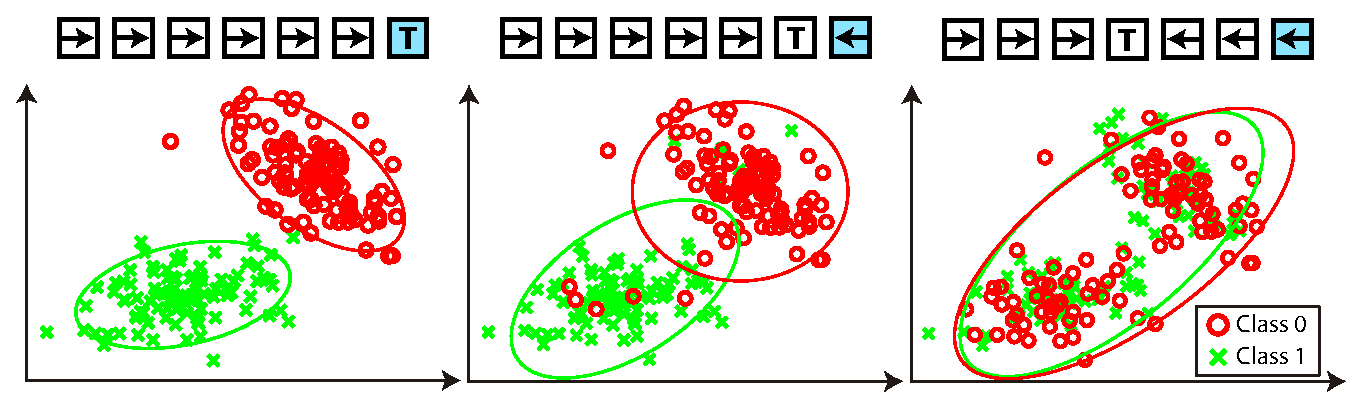
\includegraphics[width=\columnwidth]{img/real_vs_fake.eps}
%\caption{Hypothesis label spaces for a 1D grid world. For the represented example, the arrows indicate for each state what action should elicit a positive feedback to reach the state marked with T (i.e., the optimal policies). Below are shown the received signals (represented as points in a 2D feature space) labeled according to their respective task hypothesis. Corresponding 2D Gaussian distributions estimates are overlaid. While for the correct target (shaded blue state) the distributions shows a large separability (Left), the overlaps increases as the believed target moves away from the real one (Middle, Right).}
%\label{fig:intuition}
%\end{figure}
%



% Perceptual learning and task learning can both benefit from user interaction in many different ways. On the one hand, if the interaction protocol and context, is well defined it is possible to acquired grounded perceptual data. On the other hand, if the human and the machine understand each others, the human can explain or guide the machine, which may reduce learning time or even enable the machine to learn task difficult to write down as an objective or reward function.


% Machine-learning and artificial intelligence research aims at giving computers the ability to learn without being explicitly told. Two widely explored subfields are perceptual learning, in which the system learns to discriminate between perceptual events, and task learning, in which the system learn to increase its performance wrt. an objective or a reward function. 
% Well known results include hand writing recognition \todo{cite}, scene analysis \todo{cite} on the perceptual learning side and \todo{stuff} on the task learning side.

% For long most of the task learning research focused on abstract, well structure, problems. More recently, machine and in particular machines, are \todo{believed to be useful in our daily life}. Such machine will need the ability to learn new task in open-ended environment were an objective or reward function is not easy to define. Current approaches consist of inferring the reward function by interacting with others (e.g. humans) who already acquired the skill. \todo{This field is known as learning from demonstration. Inverse Reinforcement Learning is.}

% However most of those systems have not considered in depth the properties of teaching interactions with a human in the loop. This issues have began to be addressed in works studying interactive learning \todo{cite}, which combines the ideas of learning from demonstration, learning by exploration and tutor feedback.

% Recently interactive learning as acquired increasing attention.

%Under this approach, the teacher interacts with the machine and provides extra feedback or guidance. In addition, the machine can act to improve its learning efficiency. Recent developments have considered: extra reinforcement signals \todo{cite}, action requests \todo{cite}, disambiguation among actions \todo{cite}, preferences among states \todo{cite}, iterations between practice and user feedback sessions \todo{cite} and choosing actions that maximise the user feedback \todo{cite}.

% Perceptual learning and task learning can both benefit from user interaction in many different ways. On the one hand, if the interaction protocol and context, is well defined it is possible to acquired grounded perceptual data. On the other hand, if the human and the machine understand each others, the human can explain or guide the machine, which may reduce learning time or even enable the machine to learn task difficult to write down as an objective or reward function.

% While impressive results have been obtained in each domain, 
% However most work considered them separately:
% \begin{itemize} 
% \item In perceptual learning from human interaction perceptual events are learned to be categorized. The human provides signals related to some perceptual events. Associating perception and human signals implies \textbf{the machine is aware of the communicative goal of the human}.
% associated to their respective names.
% human 's communicative signals are learn to be associated to their respective meanings. 
% Such learning often rely on supervised classification methods, which implies collecting data samples associated with their respective names (called labels), which are provided by the human partners. This latter requirement implies \textbf{the machine is aware of the communicative goal of the human}.
% \item In task learning from human interaction most work has focused on how to extract statistical task models from human teaching signals. Therefore a usual assumption is that \textbf{the machine understands the meanings of human' s  communicative signals}.
% \end{itemize}


% The system is updating as many models as task hypothesis and is looking for the one from which emerges a coherence in the prediction of the user signals by the classifier and the expected meanings from the hypothesis.


% \todo{In machine learning terms, given the dataset of signals $e$, the best set of labels is the one producing the classifier of best accuracy. In other words, we will select the set which display a more coherent structure between the labels and the spacial organization of signals, according to the assumptions, constraints and biases of the classification algorithm used.}

% An intuition on how the algorithm works is to imagine the agent assigning hypothetic labels (i.e. meanings) to signals for each possible task. The system is updating as many models as task hypothesis and is looking for the one from which emerges a coherence in the prediction of the user signals by the classifier and the expected meanings from the hypothesis.


% An important consequence of this algorithm is that once a first task has been identified correctly, the true label of the received signals are known. Hence, once a first task has been learnt from scratch, it becomes equivalent to a calibration procedure, and the next task to be learn will be similar to a task learning problem from known signal to meaning mapping learnt from a calibration procedure. \todo{it is even improved}






% We call this problem learning from unlabelled interaction frame or joint perceptual and task learning.
%
% Frames are a concept that emerges simultaneously in social theory \cite{goffman1974frame} and artificial intelligence \cite{minsky1974framework}. They represents a stereotyped situations, a schema of interpretation given a particular situation or event. It is answering the question: \emph{what is going on here ?},  in order to reduce ambiguity of intangible topics by contextualizing the information.
%
% Interaction frames are the subclass of frames that account for interaction scenario. A simple interaction frame would be a human providing discrete action advice to a machine in the context of a reaching task. Being aware of this frame, the machine knows the utterances of the user correspond to action it should perform to achieve user intended goal. In task learning, such frame is often assumed to be known by both the human and the machine in addition to the signal-to-meaning classifier that translate the actual user signal into meaningful symbols.
%
%A simple interaction frame would be a human presenting an object to a machine at the same time as saying the name of the object. Being aware of this frame, the machine knows the utterance correspond to the name of the object (and not its shape or color). In others words the label of the speech signal is given.
%
% An unlabelled interaction frames correspond to a loosely defined interaction frame in which the interactive partners knows what kind of signal to expect but not the particular details of it. Following our example, a loosely defined frame would be cases where the signal-to-meaning classifier is unknown to the machine. What remains is the fact the interaction is constrained, and the user is known to deliver signal that correspond to desired action from the machine in order to achieve a task. In other word the label of the unknown speech signal is not explicitly given but is known to belong to one of a finite set of possible meanings.
%the human saying either the name, the color or the shape of the object.
%
% Such unlabelled interaction frame is at the core of our approach, it is assumed to be known by both the human and the machine in order for our algorithm to work. It includes both the context in which the interaction in taking place, e.g. teaching a machine which state to reach in the world, and the protocol used by the teacher to communicate to the machine, e.g. the teacher assessing machine's action.

% The problem we want to solve resumes in trying to learn what to do without knowing what we are told to do. 
